\hypertarget{rendererdata_8cpp}{}\section{Файл Projects/labs/course\+\_\+project\+\_\+cg/src/animation/rendererdata.cpp}
\label{rendererdata_8cpp}\index{Projects/labs/course\+\_\+project\+\_\+cg/src/animation/rendererdata.\+cpp@{Projects/labs/course\+\_\+project\+\_\+cg/src/animation/rendererdata.\+cpp}}
{\ttfamily \#include \char`\"{}renderdata.\+h\char`\"{}}\\*
Граф включаемых заголовочных файлов для rendererdata.\+cpp\+:\nopagebreak
\begin{figure}[H]
\begin{center}
\leavevmode
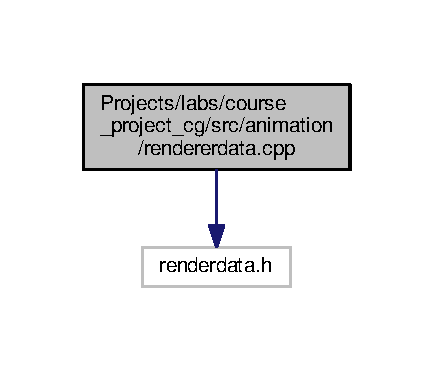
\includegraphics[width=208pt]{de/da3/rendererdata_8cpp__incl}
\end{center}
\end{figure}
